\documentclass[letterpaper]{article}
%------------------------------------------------------------------------------------------
\title{Equations and Derivations for the Quaternion Python Module}
\author{Philippe Pinard}
\date{\today}
%------------------------------------------------------------------------------------------
\usepackage[letterpaper,top=2.5cm,bottom=2.5cm,right=2.5cm,left=2.5cm]{geometry}
\usepackage[english]{babel}
\usepackage[latin1]{inputenc}
%------------------------------------------------------------------------------------------
%\usepackage{fullpage}
\usepackage{graphicx}
\usepackage{subfigure}
\usepackage{multirow}
\usepackage{url}
\usepackage{amsmath}
\usepackage{amsfonts}
\usepackage{stmaryrd}
\usepackage{setspace}
\usepackage{sistyle}
\usepackage[nothing]{todo}
\usepackage[version=3]{mhchem}
\usepackage{fancyhdr}
\usepackage{paralist}
\usepackage{epic}
\usepackage{array}
%------------------------------------------------------------------------------------------
\usepackage[
	pdftitle={Equations and Derivations for the Pattern Simulations Python Module},
	pdfsubject={Programming notes},
	pdfkeywords ={pattern, lines, bands, plane spacing, Python, Derivations},
	pdfauthor={Philippe Pinard},
	colorlinks=true,
	linkcolor=blue,
	pdfborder=0 0 0,
	pdfhighlight=/I,
	pdfpagelabels]{hyperref}
%------------------------------------------------------------------------------------------

\DeclareMathAlphabet{\mathpzc}{OT1}{pzc}{m}{it}
\newcommand{\dev}{\ensuremath{\ \mathrm{d}}}
\renewcommand{\labelitemii}{$\diamond$}
\newcommand{\celsius}{^\circ C}
\renewcommand{\tablename}{Table}
\renewcommand{\figurename}{Figure}
\newcommand{\conj}[1]{#1^\ast}
\newcommand{\trans}[1]{#1^\mathrm{T}}
\newcommand{\vx}{\hat{x}}
\newcommand{\vy}{\hat{y}}
\newcommand{\vz}{\hat{z}}
\newcommand{\trace}[1]{\mathrm{Tr}(#1)}
\newcommand{\quaternion}[2]{\llbracket #1, #2 \rrbracket}
\newcommand{\quaternionL}[1]{\mathcal{#1}}
\newcommand{\norm}[1]{\left\|#1\right\|}
\newcommand{\im}{\mathit{i}}
\newcommand{\direction}[1]{\left[ #1 \right]}
\newcommand{\vecc}[3]{\left(#1,#2,#3\right)}
\newcommand{\var}[1]{\mathpzc{#1}}

\begin{document}
%------------------------------------------------------------------------------------------
	\pagestyle{fancy}
	\fancyhf{}
	\setlength{\headheight}{15pt}
	\setlength{\headsep}{10pt}
	\lhead{Equations and Derivations for the Pattern Simulations Python Module}
	\rhead{\today}
	\lfoot{\emph{Prepared by Philippe Pinard}}
	\rfoot{\thepage}
%------------------------------------------------------------------------------------------
	
	\section{Definitions and Notations}
	\subsection{Abbreviations}
		\begin{itemize}
			\item $\var{WD}$: Working Distance
			\item $\var{PC}$: Pattern center ($\var{PC}_x$: x coordinates of the pattern center)
			\item $\var{DD}$: Detector distance
			\item $hkl$: Plane coordinates
			\item $\vx$, $\vy$, $\vz$: Unit vectors of the reference axis system
		\end{itemize}
	\subsection{Reference Coordinates System}
		\begin{tabular}{p{0.3\textwidth}p{0.3\textwidth}p{0.3\textwidth}}
			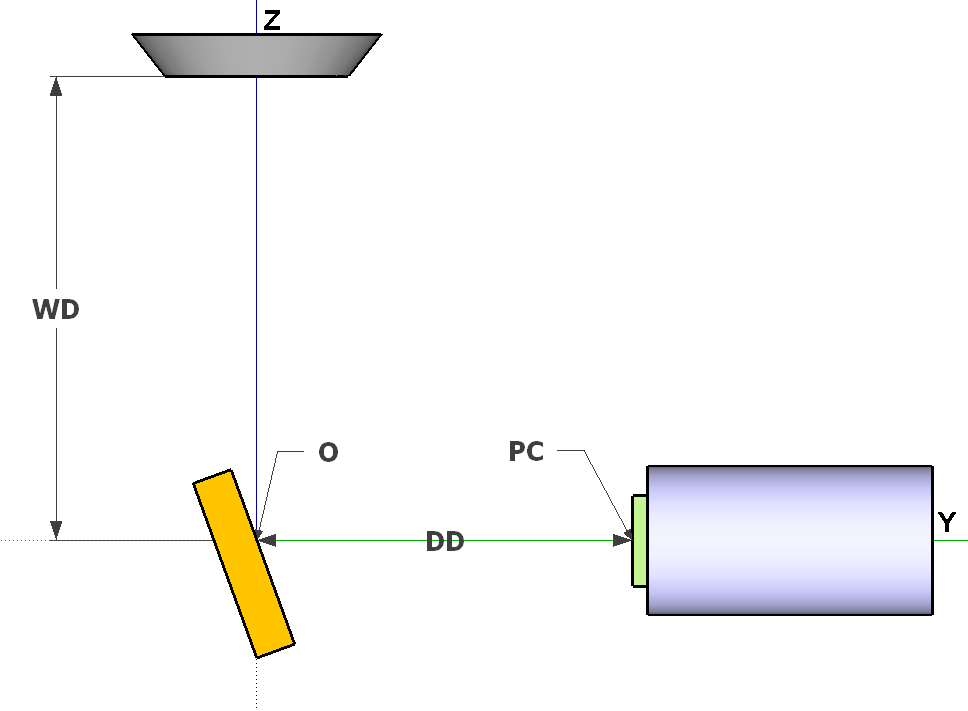
\includegraphics[width=0.3\textwidth]{figures/axis_system1} & 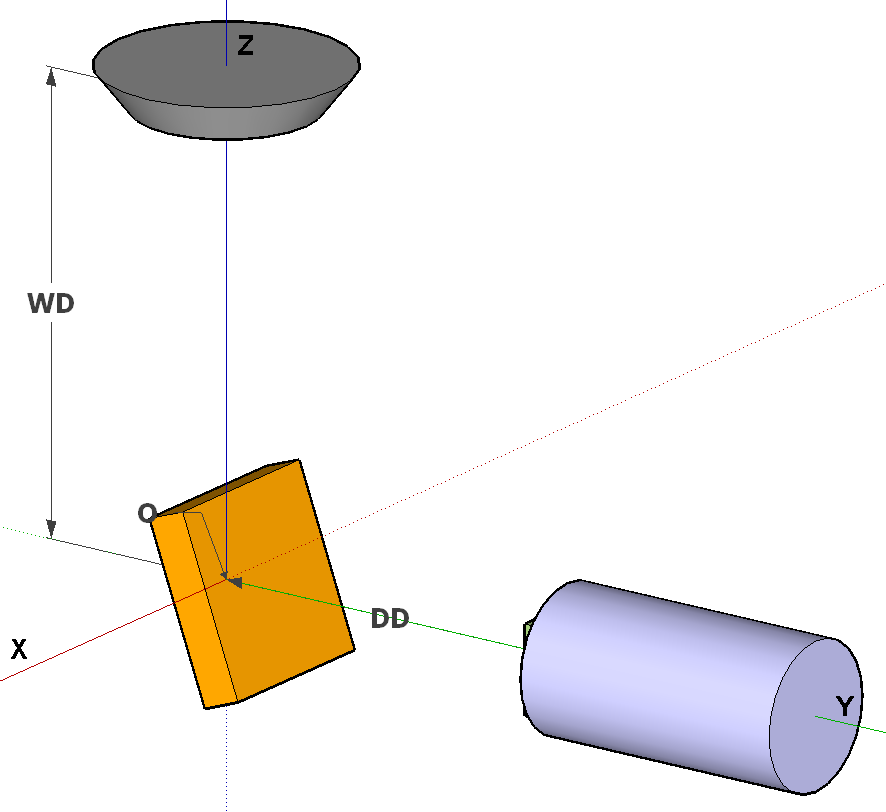
\includegraphics[width=0.3\textwidth]{figures/axis_system2} & 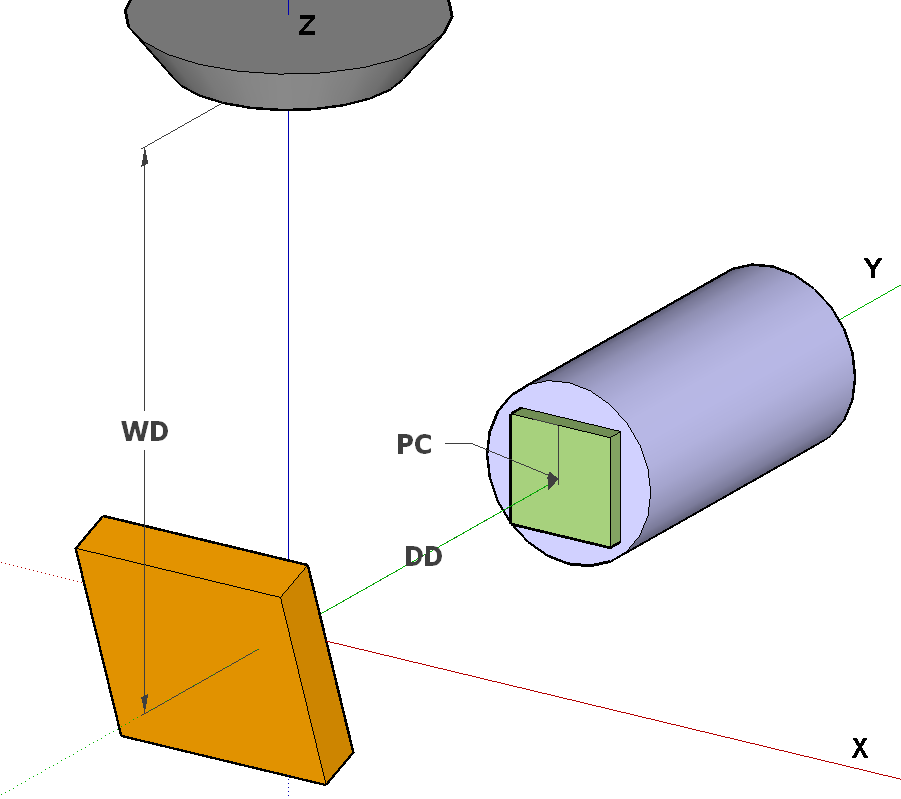
\includegraphics[width=0.3\textwidth]{figures/axis_system3} 
		\end{tabular}
		\begin{itemize}
			\item The origin is taken as the point where the beam intersects the sample. To be more precise, the top left corner of the acquisition map.
			\item The default position of the detector (i.e.\ without any correction of the detector orientation) is at $\var{DD}\vy$ of the sample.
			\item The default tilt axis is along the $\vx$ axis. Counter-clockwise rotation are taken as positive rotation.
			\item The coordinates of the $\var{PC}$ are $(\var{PC}_x, \var{DD}, \var{PC_z})$.
		\end{itemize}
	
	\section{Planes to Kikuchi bands}
	From planes representing a particular crystallographic orientation to their representations as Kikuchi bands on the detector, several steps are involved:
	\begin{enumerate}
		\item Reference coordinates system $\xrightarrow{\text{Specimen orientation}}$ Specimen coordinates system
		\item Specimen coordinates system $\xrightarrow{\text{Crystal orientation}}$ Crystal coordinates system
		\item Crystal coordinates system $\xrightarrow{\text{Tilt}}$ Tilted coordinates system
		\item Tilted coordinates system $\xrightarrow{\text{Detector orientation}}$ Detector corrected or Diffraction coordinates system
		\item Diffraction coordinates system $\rightarrow{\text{Diffraction}}$ Kikuchi bands
	\end{enumerate}
	
	\subsection{Specimen orientation}
	
	
	\subsection{Crystal orientation}
	
	\subsection{Tilt}
	
	
	\subsection{Detector orientation}
	
	\subsection{Diffraction}
	\subsubsection{Kikuchi Line}
	For a plane with a normal $\vec{n} = (n_x, n_y, n_z)$ and passing through the origin, the plane equation is:
	\begin{eqnarray}
		\vec{n} \cdot (x,y,z) & = & 0\\\nonumber
		n_xx + n_yy + n_zz & = & 0 
		\label{eq:plane}
	\end{eqnarray}
	
	Kikuchi lines (center of the Kikuchi bands) represent the intersection of diffracting planes with the detector.  
	This intersection of a plane with another plane is a line.
	To find the intersect of this plane, we can replace $(x,y,z)$ in Equation~\ref{eq:plane} by $(x, \var{DD}, z)$ since $y$ is fixed at $\var{DD}$ and write the line equation.
	\begin{eqnarray}
		n_x x + n_y \var{DD} + n_z z = 0 \\\nonumber
		z = -\frac{n_x}{n_z}x - \frac{n_y}{n_z}\var{DD}
		\label{eq:plane2}
	\end{eqnarray}
	
	Equation~\ref{eq:plane2} is incomplete, because it doesn't take into account the position of the pattern center, which might not be located at $(0,\var{DD},0)$. 
	For this correction, $x$ becomes $x-\var{PC}_x$ and $z$, $z-\var{PC}_z$.
	Rewriting the equation, we obtain:
	\begin{eqnarray}
		z = \left(-\frac{n_x}{n_z}\right)x + \left(\frac{n_x}{n_z}\var{PC}_x + - \frac{n_y}{n_z}\var{DD} + \var{PC}_z\right)
		\label{eq:plane3}
	\end{eqnarray}
	
	The slope is therefore $m=-\frac{n_x}{n_z}$ and the intercept $b=\frac{n_x}{n_z}\var{PC}_x + - \frac{n_y}{n_z}\var{DD} + \var{PC}_z$. 
	Equation~\ref{eq:plane3} is undetermined when $n_z = 0$. 
	This situations corresponds to a vertical line $x = \text{constant}$.
	\begin{eqnarray}
		n_x x + n_y \var{DD} + (0) z = 0 \\\nonumber
		x = -\frac{n_y}{n_x}\var{DD} + \var{PC}_x
		\label{eq:plane4}
	\end{eqnarray}
	
	Again there is a special case when $n_z = 0$ and $n_x = 0$, which corresponds to a plane parallel to the detector's plane. 
	There is no Kikuchi band for this case.
	
	\subsubsection{Kikuchi Bands}
	To determine the width of the Kikuchi Bands, we need to determine the scattering angle $\theta$ using the Bragg's Law. The wavelength $\lambda$ is determined from the electron's incident energy, and the plane spacing $d$ from the lattice parameters.
	\begin{eqnarray}
		\lambda = 2d\sin\theta
		\label{eq:bragg}
	\end{eqnarray}
	
	
	The scattering angle creates two Kikuchi cones (Figure~\ref{}). 
	It is the intersection of these cones with the detector that gives a width to the Kikuchi bands.
	The intersection of cones with a planes gives an hyperbola. 
	However, since the scattering angle is small for electron energies used in SEM, the hyperbola can be approximated as two lines. 
	So, to simplify the calculations, the cones are replaced by two planes separated by an angle $2\theta$.
	
	
	To convert the scattering angle $\theta$  to a distance on the detector $w$, we first find the smallest distance between the Kikuchi line and the origin. 
	This distance would correspond to half the distance between the two inflexion points of the hyperbola.
	This distance between a line and a point is given by Equation~\ref{eq:pointline}\ref{mathworld}, where $\vec{x_0}$ is the point, and $\vec{x_1}$ and $\vec{x_2}$ are two points on the line.
	\begin{eqnarray}
		d = \frac{\norm{(\vec{x_2}-\vec{x_1}) \times (\vec{x_1}-\vec{x_0})}}{\norm{\vec{x_2}-\vec{x_1}}}
		\label{eq:pointline}
	\end{eqnarray}
	One can notice that the numerator is in fact the normal $\vec{N}$ of the plane formed by $\vec{x_0}$, $\vec{x_1}$ and $\vec{x_2}$.
	
	
	
	
\end{document}

		
%	\begin{picture}(300,200)
%		%Axis 3D
%%		\put(10,10){\vector(0,1){20}}
%%		\put(10,10){\vector(1,0){20}}
%%		\put(10,10){\vector(-1,-1){10}}
%%		\put(13,25){\small{$z$}}
%%		\put(25,3){\small{$y$}}
%%		\put(-2,5){\small{$x$}}
%		\includegraphics[width=0.5\textwidth]{figures/axis_system}
%		%Axis 2D
%		\put(10,10){\vector(0,1){20}}
%		\put(10,10){\vector(1,0){20}}
%		\put(6,7.5){$\varotimes$}
%		\put(13,25){\small{$z$}}
%		\put(25,3){\small{$y$}}
%		\put(2,2){\small{$x$}}
%		
%		
%	\end{picture}
%	